%set the master document for easy compilation
%!TEX root = ../D3_5_2.tex

\section{Train\_Supervision}

\subsection{Component Requirements}

\begin{longtable}{p{.25\textwidth}p{.7\textwidth}}
\toprule
Component name			& TrainSupervision \\
\midrule
Link to SCADE model		& {\footnotesize \url{???}} \\
\midrule
SCADE designer			& Christian Stahl, TWT \\
\midrule
Description				& The task of block ``Train Supervision'' is to monitor the speed of the train and the train location and as such to ensure that the speed remains within the given speed and distance limits. This block is mainly based on \cite[Chapt.~3.13]{subset-026}.

The block ``Train Supervision'' takes as input (1) movement related information such as train speed, train position and acceleration, (2) train related information such as brake information and train length, and (3) track related information such as speed and distance limits and national values.

Based on this information a speed profile is calculated. Speed restrictions create target speeds (targets) that have to be followed. For each such target braking curves are generated to supervise at which location of the track the train must perform the brake. In case of no target restrictions the train may accelerate to the supervised maximum speed of the speed profile. These calculations lead to commands being sent to the driver and the brake system.

The functionality is modeled using eight operators, as shown in Figure~\ref{f:ssv}, which are explained below.

The current status of the analysis of ``Train Supervision'' and a functional breakdown can be found in a separate document, \verb+SpeedSupervision_analysis.pdf+.\\
\midrule
Input documents	& 
Subset-026, Chapter 3.13: Speed and distance monitoring \\
\midrule
Safety integrity level		& 4 \\
\midrule
Time constraints		& [If applicable description of time constraints, otherwise n/a] \\
\midrule
API requirements 		& [If applicable description of API requirements, otherwise n/a] \\
\bottomrule
\end{longtable}


\subsection{Interface}

An overview of the interface of component [component name] is shown in Figure~\ref{f:ssv}. The inputs and outputs are described in detail in Section~\ref{s:template_inputs} respectively \ref{s:template_outputs}.

\begin{figure}
\centering
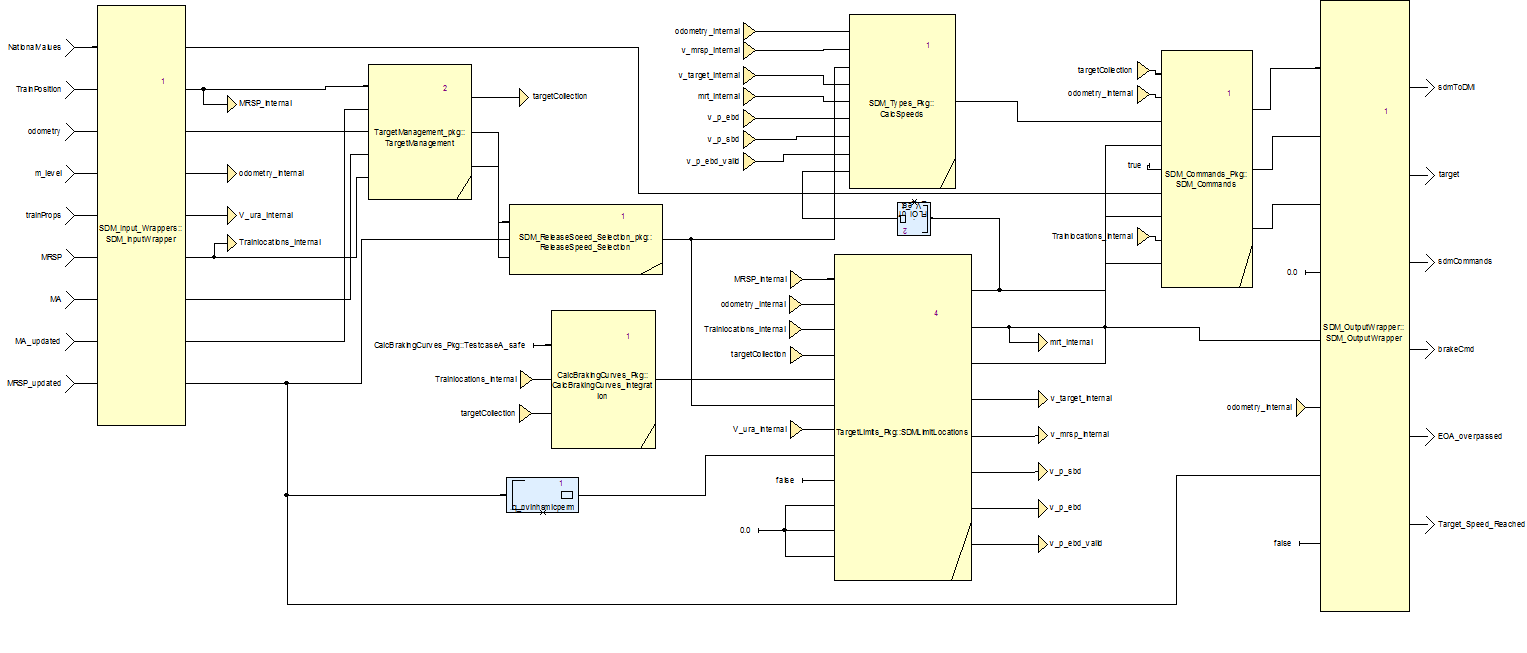
\includegraphics[width=0.95\textheight, angle=90]{../images/speedsupervision.png}
\caption{Structure of component ProvidePositionReport.}\label{f:ssv}
\end{figure}



\subsubsection{Inputs}\label{s:template_inputs}

\paragraph{NationalValues}

\begin{longtable}{p{.25\textwidth}p{.7\textwidth}}
\toprule
Input name				& NationalValues \\
\midrule
Description				& This input is packet 3 of \cite[Chapt.~8]{subset-026}, describing the national values.  \\
\midrule
Source					& ??? \\ 
\midrule
Type					& P3\_NationalValues\_T \\
\midrule
Valid range of values	& [Complete list of valid values] \\
\midrule
Behaviour when value is at boundary	& [Description of components behaviour when input value is at boundary] \\
\midrule
Behaviour for values out of valid range	& [Description of components behaviour when input value is out of valid range] \\
\bottomrule
\end{longtable}


\paragraph{TrainPosition}

\begin{longtable}{p{.25\textwidth}p{.7\textwidth}}
\toprule
Input name				& TrainPosition \\
\midrule
Description				& This input is the current train position. \\
\midrule
Source					& Manage Track Data \\ 
\midrule
Type					& trainPosition\_T \\
\midrule
Valid range of values	& [Complete list of valid values] \\
\midrule
Behaviour when value is at boundary	& [Description of components behaviour when input value is at boundary] \\
\midrule
Behaviour for values out of valid range	& [Description of components behaviour when input value is out of valid range] \\
\bottomrule
\end{longtable}


\paragraph{odometry}

\begin{longtable}{p{.25\textwidth}p{.7\textwidth}}
\toprule
Input name				& odometry \\
\midrule
Description				& This input is the odometry data. \\
\midrule
Source					& Odometry \\ 
\midrule
Type					& odometry\_T \\
\midrule
Valid range of values	& [Complete list of valid values] \\
\midrule
Behaviour when value is at boundary	& [Description of components behaviour when input value is at boundary] \\
\midrule
Behaviour for values out of valid range	& [Description of components behaviour when input value is out of valid range] \\
\bottomrule
\end{longtable}\chapter{[Input 2 name]}


\paragraph{m\_level}

\begin{longtable}{p{.25\textwidth}p{.7\textwidth}}
\toprule
Input name				& m\_level \\
\midrule
Description				& This input is the current level of the train. \\
\midrule
Source					& Mode and Level \\ 
\midrule
Type					& M\_LEVEL \\
\midrule
Valid range of values	& [Complete list of valid values] \\
\midrule
Behaviour when value is at boundary	& [Description of components behaviour when input value is at boundary] \\
\midrule
Behaviour for values out of valid range	& [Description of components behaviour when input value is out of valid range] \\
\bottomrule
\end{longtable}\chapter{[Input 2 name]}

\paragraph{trainProps}

\begin{longtable}{p{.25\textwidth}p{.7\textwidth}}
\toprule
Input name				& trainProps \\
\midrule
Description				& This input is a set of train related properties. \\
\midrule
Source					& Database \\ 
\midrule
Type					& trainProperties\_T \\
\midrule
Valid range of values	& [Complete list of valid values] \\
\midrule
Behaviour when value is at boundary	& [Description of components behaviour when input value is at boundary] \\
\midrule
Behaviour for values out of valid range	& [Description of components behaviour when input value is out of valid range] \\
\bottomrule
\end{longtable}\chapter{[Input 2 name]}


\paragraph{MRSP}

\begin{longtable}{p{.25\textwidth}p{.7\textwidth}}
\toprule
Input name				& MRSP \\
\midrule
Description				& This input is the most restrictive speed profile. \\
\midrule
Source					& ??? \\ 
\midrule
Type					& MRSP\_Profile\_t \\
\midrule
Valid range of values	& [Complete list of valid values] \\
\midrule
Behaviour when value is at boundary	& [Description of components behaviour when input value is at boundary] \\
\midrule
Behaviour for values out of valid range	& [Description of components behaviour when input value is out of valid range] \\
\bottomrule
\end{longtable}\chapter{[Input 2 name]}


\paragraph{MA}

\begin{longtable}{p{.25\textwidth}p{.7\textwidth}}
\toprule
Input name				& MA \\
\midrule
Description				& This input is a movement authority. \\
\midrule
Source					& ??? \\ 
\midrule
Type					& MAs\_t \\
\midrule
Valid range of values	& [Complete list of valid values] \\
\midrule
Behaviour when value is at boundary	& [Description of components behaviour when input value is at boundary] \\
\midrule
Behaviour for values out of valid range	& [Description of components behaviour when input value is out of valid range] \\
\bottomrule
\end{longtable}\chapter{[Input 2 name]}


\paragraph{MA\_updated}

\begin{longtable}{p{.25\textwidth}p{.7\textwidth}}
\toprule
Input name				& MA\_updated \\
\midrule
Description				& This flag is true if the movement authority has been updated in this clock cycle and false otherwise. \\
\midrule
Source					& internal \\ 
\midrule
Type					& bool \\
\midrule
Valid range of values	& [Complete list of valid values] \\
\midrule
Behaviour when value is at boundary	& [Description of components behaviour when input value is at boundary] \\
\midrule
Behaviour for values out of valid range	& [Description of components behaviour when input value is out of valid range] \\
\bottomrule
\end{longtable}


\paragraph{MRSP\_updated}

\begin{longtable}{p{.25\textwidth}p{.7\textwidth}}
\toprule
Input name				& MRSP\_updated \\
\midrule
Description				& This flag is true if the most restrictive speed profile has been updated in this clock cycle and false otherwise. \\
\midrule
Source					& internal \\ 
\midrule
Type					& bool \\
\midrule
Valid range of values	& [Complete list of valid values] \\
\midrule
Behaviour when value is at boundary	& [Description of components behaviour when input value is at boundary] \\
\midrule
Behaviour for values out of valid range	& [Description of components behaviour when input value is out of valid range] \\
\bottomrule
\end{longtable}


\subsubsection{Outputs}\label{s:template_outputs}

\paragraph{sdmToDMI}

\begin{longtable}{p{.25\textwidth}p{.7\textwidth}}
\toprule
Output name				& sdmToDMI \\
\midrule
Description				& This output contains information about different speeds and positions, on the one hand and the current supervision status, on the other hand. This information shall be displayed to the driver. \\
\midrule
Destination				& [Name of the destination component(s)] \\ 
\midrule
Type					& speedSupervisionForDMI\_T \\
\midrule
Valid range of values	& [Complete list of valid values] \\
\midrule
Behaviour when value is at boundary	& [Description of components behaviour when output value is at boundary] \\
\midrule
Behaviour for values out of valid range	& [Description of components behaviour when output value is out of valid range] \\
\bottomrule
\end{longtable}


\paragraph{target}

\begin{longtable}{p{.25\textwidth}p{.7\textwidth}}
\toprule
Output name				& target \\
\midrule
Description				& This output is the most restrictive displayed target (MRDT). \\
\midrule
Destination				& [Name of the destination component(s)] \\ 
\midrule
Type					& Target\_T \\
\midrule
Valid range of values	& [Complete list of valid values] \\
\midrule
Behaviour when value is at boundary	& [Description of components behaviour when output value is at boundary] \\
\midrule
Behaviour for values out of valid range	& [Description of components behaviour when output value is out of valid range] \\
\bottomrule
\end{longtable}


\paragraph{sdmCommands}

\begin{longtable}{p{.25\textwidth}p{.7\textwidth}}
\toprule
Output name				& sdmCommands \\
\midrule
Description				& This output gives some intermediate results of operator SDM\_Commands. It is currently used for test purposes only. \\
\midrule
Destination				& [Name of the destination component(s)] \\ 
\midrule
Type					& SDM\_Commands\_T \\
\midrule
Valid range of values	& [Complete list of valid values] \\
\midrule
Behaviour when value is at boundary	& [Description of components behaviour when output value is at boundary] \\
\midrule
Behaviour for values out of valid range	& [Description of components behaviour when output value is out of valid range] \\
\bottomrule
\end{longtable}

\paragraph{brakeCmd}

\begin{longtable}{p{.25\textwidth}p{.7\textwidth}}
\toprule
Output name				& brakeCmd \\
\midrule
Description				& This output is the brake command, indicating whether performing the service brake or the emergency brake have been commanded. \\
\midrule
Destination				& [Name of the destination component(s)] \\ 
\midrule
Type					& Brake\_command\_T \\
\midrule
Valid range of values	& [Complete list of valid values] \\
\midrule
Behaviour when value is at boundary	& [Description of components behaviour when output value is at boundary] \\
\midrule
Behaviour for values out of valid range	& [Description of components behaviour when output value is out of valid range] \\
\bottomrule
\end{longtable}


\paragraph{EOA\_overpassed}

\begin{longtable}{p{.25\textwidth}p{.7\textwidth}}
\toprule
Output name				& EOA\_overpassed \\
\midrule
Description				& This output is true if the end of authority has been overpassed and false otherwise. \\
\midrule
Destination				& [Name of the destination component(s)] \\ 
\midrule
Type					& bool \\
\midrule
Valid range of values	& [Complete list of valid values] \\
\midrule
Behaviour when value is at boundary	& [Description of components behaviour when output value is at boundary] \\
\midrule
Behaviour for values out of valid range	& [Description of components behaviour when output value is out of valid range] \\
\bottomrule
\end{longtable}


\paragraph{Target\_Speed\_Reached}

\begin{longtable}{p{.25\textwidth}p{.7\textwidth}}
\toprule
Output name				& Target\_Speed\_Reached \\
\midrule
Description				& This output is true if the current speed is greater than or equal the target speed and false otherwise. \\
\midrule
Destination				& [Name of the destination component(s)] \\ 
\midrule
Type					& bool \\
\midrule
Valid range of values	& [Complete list of valid values] \\
\midrule
Behaviour when value is at boundary	& [Description of components behaviour when output value is at boundary] \\
\midrule
Behaviour for values out of valid range	& [Description of components behaviour when output value is out of valid range] \\
\bottomrule
\end{longtable}